\documentclass{beamer}

\usepackage{color} % Package to include colors for syntax highlighting
\usepackage{graphicx}  % Package to include images
\usepackage{hyperref}  % Hyperlinks
\usepackage{tikz}
\usepackage{minted}

\setbeamertemplate{navigation symbols}{}  % Remove navigation symbols
\usecolortheme[light]{solarized}

\title{Computing for Mathematics: Week 1}
\date{}


\begin{document}

\frame{
    \titlepage
}

\frame{
    \frametitle{Vince Knight}

    \begin{itemize}
        \item Office: M1.30
        \item email: knightva@cf.ac.uk
        \item Office hours: Thursday 1300 - 1500
        \item \url{vknight.org/cfm}
    \end{itemize}

}

\frame{
    \begin{center}
        \includegraphics[width=.5\textwidth]{img/gauss.png}
        \pause

        (Gauss, 1777-1855)
    \end{center}
}

\frame{
    \Huge
\[\sum_{i=0}^{100}i\]
}

\frame{
    \frametitle{Cryptography:}
    \begin{center}
        \url{https://www.youtube.com/watch?v=_i-TcU0zLE0}
    \end{center}
}

\frame{
    \frametitle{Programming and Mathematics}

    There are various areas in which computers are of major importance to Mathematicians:

    \begin{itemize}
        \item Computer assisted proofs;
        \item Implementation of mathematics;
        \item Computer generated proofs;
        \item Everyday mathematics.
    \end{itemize}

}

\frame{
    \frametitle{Computer assisted proofs}

    \begin{center}

        \begin{tikzpicture}

            \only<1>{
                \node (A) [circle, draw] at (-.5,2) {0};
                \node (B) [circle, draw] at (0,1) {1};
                \node (C) [circle, draw] at (1.5,2) {2};
                \node (D) [circle, draw] at (-.5,0) {3};
                \node (E) [circle, draw] at (2,.7) {4};
            }

            \only<2>{
                \node (A) [circle, draw, fill=blue] at (-.5,2) {0};
                \node (B) [circle, draw] at (0,1) {1};
                \node (C) [circle, draw] at (1.5,2) {2};
                \node (D) [circle, draw] at (-.5,0) {3};
                \node (E) [circle, draw] at (2,.7) {4};
            }

            \only<3>{
                \node (A) [circle, draw, fill=blue] at (-.5,2) {0};
                \node (B) [circle, draw, fill=green] at (0,1) {1};
                \node (C) [circle, draw] at (1.5,2) {2};
                \node (D) [circle, draw] at (-.5,0) {3};
                \node (E) [circle, draw] at (2,.7) {4};
            }

            \only<4>{
                \node (A) [circle, draw, fill=blue] at (-.5,2) {0};
                \node (B) [circle, draw, fill=green] at (0,1) {1};
                \node (C) [circle, draw, fill=red] at (1.5,2) {2};
                \node (D) [circle, draw, fill=red] at (-.5,0) {3};
                \node (E) [circle, draw] at (2,.7) {4};
            }

            \only<5-6>{
                \node (A) [circle, draw, fill=blue] at (-.5,2) {0};
                \node (B) [circle, draw, fill=green] at (0,1) {1};
                \node (C) [circle, draw, fill=red] at (1.5,2) {2};
                \node (D) [circle, draw, fill=red] at (-.5,0) {3};
                \node (E) [circle, draw, fill=gray] at (2,.7) {4};
            }
            \draw (A) -- (C);
            \draw (A) -- (B);
            \draw (A) -- (D);
            \draw (A) -- (E);
            \draw (B) -- (C);
            \draw (B) -- (E);
            \draw (B) -- (D);
            \draw (E) -- (D);
            \draw (E) -- (C);
        \end{tikzpicture}
    \end{center}

    \begin{itemize}
            \onslide<5-6>{
            \item `4 colour theorem': \textbf{Any map can be coloured using 4 colours.\\}
            }

            \onslide<6>{

            \item Proved in 1976 by Kenneth Appel and Wolfgang Haken:
                \begin{center}
                    \framebox{Used computers to check 1936 particular cases.}
                \end{center}

            }
    \end{itemize}
}

\frame{
    \frametitle{Computer assisted proofs}
    How to pack 3 dimensional spheres?

    \begin{itemize}
        \item In 1611 Kepler conjectured the best possible way.
        \item Proof in 1998 by Hales which involved a computer to minimize a function of 150 variables (100,000 times).
        \item \textbf{Also} involved a 100 page paper for the 'non computer assisted aspects'.
            \pause
        \item Referees are 99\% sure.
    \end{itemize}
}

\frame{
    \frametitle{Implementation of mathematics}
    Here at Cardiff Dr Leanne Smith studied the best way to locate ambulances in Wales. This took in to account:

    \begin{itemize}
        \item Queues;
        \item Survival probabilities of patients;
        \item Time of the day...
    \end{itemize}

    \href{http://www.youtube.com/watch?v=mMFCmd0fwjY&feature=youtu.be}{Once the mathematics was done a computer program was built to be able to demonstrate to the Welsh Ambulance Trust.}
}

\frame{
    \frametitle{Computer generated proofs}
    \begin{center}
        \href{http://goo.gl/tsdOiQ}{Timothy Gowers}
    \end{center}
    \pause
    Theorem: Let $X$ and $Y$ be sets, let $f: X \to Y$ be an injection and let $A$ and $B$ be subsetsof $X$. Then $f(A)\cap f(B)\subset f(A\cap B)$.\\

    \vspace{1cm}
    \pause
    Proof: Take $x\in f(A)\cap f(B)$. So there is some $y\in A$ and $z\in B$ such that $f(y)=f(z)=x$. As $f$ is injective, $y$ and $z$ are equal. So $y\in A\cap B$. So $x=f(y)\in f(A\cap B)$.

    \pause
    \vspace{1cm}
    The above is an example of a computer generated proof. \textbf{You do not need to know any of this!}

}

\begin{frame}[fragile]
    \frametitle{Everyday mathematics}
    Everyday mathematicians might need to calculate an integral for a bigger
    project. This is some code to calculate an integral:

    \begin{minted}{python}
sympy.integrate(x ** 3, x)
    \end{minted}

    which returns:

    $$\frac{x^4}{4}$$
\end{frame}

\frame{
    \frametitle{What we will learn}
    \begin{itemize}
        \item Python: general purpose programming (Weeks 1-5).
        \item \LaTeX:\; a package for writing mathematics (Week 6).
        \item Python: mathematical programming (Weeks 1-5).
    \end{itemize}
}

\frame{
    \begin{center}
        \url{https://www.continuum.io/downloads}
    \end{center}
}

\frame{
    \frametitle{Flipped classrooms}
    \pause
    \begin{center}
        \includegraphics[width=8cm]{img/flipped_class.png}
    \end{center}
}

\frame{
    \frametitle{Lab and Class meetings}
    \begin{itemize}
        \item Every week you have 1 class meeting to look ahead.
        \item Every week you have 1 lab sheet: you should aim to work on your
            lab sheets before the lab session.
        \item Every week you have 1 class meeting to look back and address
            difficulties.
    \end{itemize}
}

\frame{
    \begin{center}
        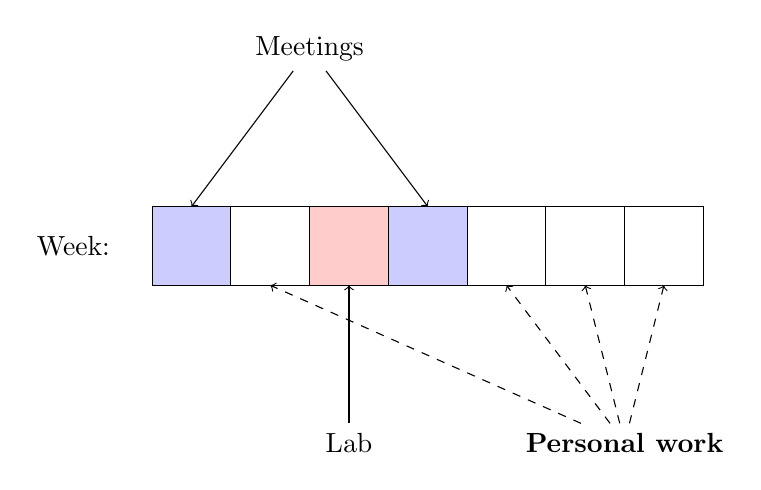
\begin{tikzpicture}
            \node at (-1, .5) {Week:};
            \draw (0, 0)  rectangle  (7, 1);

            \foreach \i in {1,...,6}
                {
                    \draw (\i, 0) -- (\i, 1);
                }

            \draw [fill=blue!20] (0, 0) rectangle (1, 1);
            \draw [fill=red!20] (2, 0) rectangle (3, 1);
            \draw [fill=blue!20] (3, 0) rectangle (4, 1);

            \node (class meetings) at (2, 3) {Meetings};

            \foreach \i in {.5, 3.5}
                {
                    \draw [->] (class meetings) -- (\i, 1);
                }

            \node (lab) at (2.5, -2) {Lab};
            \draw [->] (lab) -- (2.5, 0);

            \pause
            \node (personal work) at (6, -2) {\textbf{Personal work}};
            \foreach \i in {1.5, 4.5, 5.5, 6.5}
                {
                    \draw [dashed, ->] (personal work) -- (\i, 0);
                }

        \end{tikzpicture}
    \end{center}
}

\frame{
    \frametitle{Resources}
    \begin{center}
        \url{http://vknight.org/cfm/}
    \end{center}
}

\frame{
    \begin{center}
        \Huge Some Feedback
    \end{center}
}

\frame{\frametitle{Vince}
    \begin{quote}
        ``Vince very approachable''
    \end{quote}

    \hfill(50\%)

    \begin{quote}
        ``You are intimidating and I would personally rather approach a tutor
        for help - no offence. Where is your accent from?''
    \end{quote}

    \hfill(20\%)
}

\frame{\frametitle{The class meeting}
    \begin{quote}
        ``The lecture is useful to go over what we struggle with.''
    \end{quote}

    \hfill(60\%)

    \begin{quote}
        ``Would be better to discuss the upcoming lab sheets in lectures instead
        of the one we just did.''
    \end{quote}

    \hfill(4\%)

    \begin{quote}
        ``Some aspects should be taught first in lectures.''
    \end{quote}

    \hfill(4\%)
}

\frame{\frametitle{Labs}
    \begin{quote}
        ``Some (not all) [tutors] just give us the answers and don't explain it
        clear enough \textbf{AND}.''
    \end{quote}

    \hfill(3\%)

    \begin{quote}
        ``Sometimes asking if you're watched videos when you have is a bit
        demoralising, makes it hard to ask for help.''
    \end{quote}

    \hfill(3\%)
}

\frame{
    \begin{quote}
            ``Would like to know about all assessment from the start, class test was only recently revealed and don't know much about the remaining 45\%''
    \end{quote}
}

\frame{
    \begin{itemize}
        \item Individual Coursework: Week 11 - 70\%
        \item Group Coursework: Spring semester - 30\%
    \end{itemize}
}

\frame{
    \begin{quote}
            ``Do you have snapchat?''
    \end{quote}
}

\frame{
    \frametitle{Getting help}
    \begin{itemize}
        \item Gitter (chat) room: \url{vknight.org/cfm}.
        \item Message boards: \url{vknight.org/cfm}.
        \item email: knightva@cf.ac.uk.
        \item Office hours (M1.30): Thursday 1300 - 1500.
        \item \href{https://twitter.com/drvinceknight}{@drvinceknight} (and fb)
    \end{itemize}
}

\frame{
    \begin{center}
        \url{http://www.pydiff.wales}

        \href{https://twitter.com/pydiff}{@pydiff}
    \end{center}
}

\end{document}
